


 Rectangles $ABCD$ and $EBGH$ are inscribed in the quarter circle centered at $B$ with radius 5.  
\begin{center}
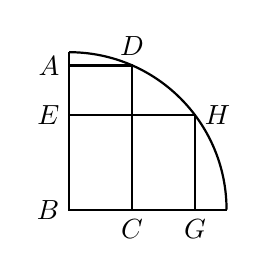
\begin{tikzpicture}
    \draw[thick] (2,0) arc (0:90:2);
    \draw[thick] (2,0)--(0,0);
    \draw[thick] (0,2)--(0,0);
   \draw[thick] (0,0) rectangle(1.6,1.2);
   \draw[thick] (0,0) rectangle(.8,1.83);
   \draw node[left] (0,0) {$B$};        
   \node[left] at (0,1.83) {$A$}; 
   \node[right] at (1.6,1.2) {$H$};
   \node[left] at (0,1.2) {$E$};
   \node[below] at (.8,0) {$C$};
   \node[above] at (.8,1.83) {$D$};
   \node[below] at (1.6,0) {$G$};
         
      
       
               
\end{tikzpicture} 
\end{center}


What is the sum of the lengths of the segments (not drawn) $\overline{AC}$ and $\overline{EG}$



\ifsat
	\begin{enumerate}[label=\Alph*)]
		\item  $5$ 
		\item  $10$ % 
		\item  $20$ 
		\item  $25$ 
	\end{enumerate}
\else
\fi

\ifacteven
	\begin{enumerate}[label=\textbf{\Alph*.},itemsep=\fill,align=left]
		\setcounter{enumii}{5}
		\item  $5$ 
		\item  $10$ % 
		\item  $15$ 
		\addtocounter{enumii}{1}
		\item  $20$ 
		\item  $25$ 
	\end{enumerate}
\else
\fi

\ifactodd
	\begin{enumerate}[label=\textbf{\Alph*.},itemsep=\fill,align=left]
		\item  $5$ 
		\item  $10$ % 
		\item  $15$ 
		\item  $20$ 
		\item  $25$ 
	\end{enumerate}
\else
\fi

\ifgridin
  $10$ % 
		
\else
\fi

